\documentclass[tikz,crop,convert={density=200,outext=.png},border=0.4cm]{standalone}

\usepackage{pgfplots}
\usepackage{amsmath}
\usetikzlibrary{arrows.meta}
\usepackage{physics}
\usepackage{xcolor}
\definecolor{clr_1}{RGB}{0,68,27}
\definecolor{clr_2}{RGB}{35,139,69}
\definecolor{clr_3}{RGB}{102,194,164}
\definecolor{clr_4}{RGB}{140,150,198}
\pgfplotsset{compat=newest,
    %width=6cm,
    %height=3cm,
    scale only axis=true,
    max space between ticks=25pt,
    try min ticks=5,
    every axis/.style={
        axis y line=middle,
        axis x line=middle,
        axis line style={thick,->,>=latex, shorten >=-.3cm}
    },
    every axis plot/.append style={thick},
    tick style={black, thick},
}
\tikzset{
    semithick/.style={line width=0.8pt},
}
\usepgfplotslibrary{groupplots}
\usepgfplotslibrary{dateplot}
% Document begins
\begin{document}
% =========================================================================================================
% Tau trans figure
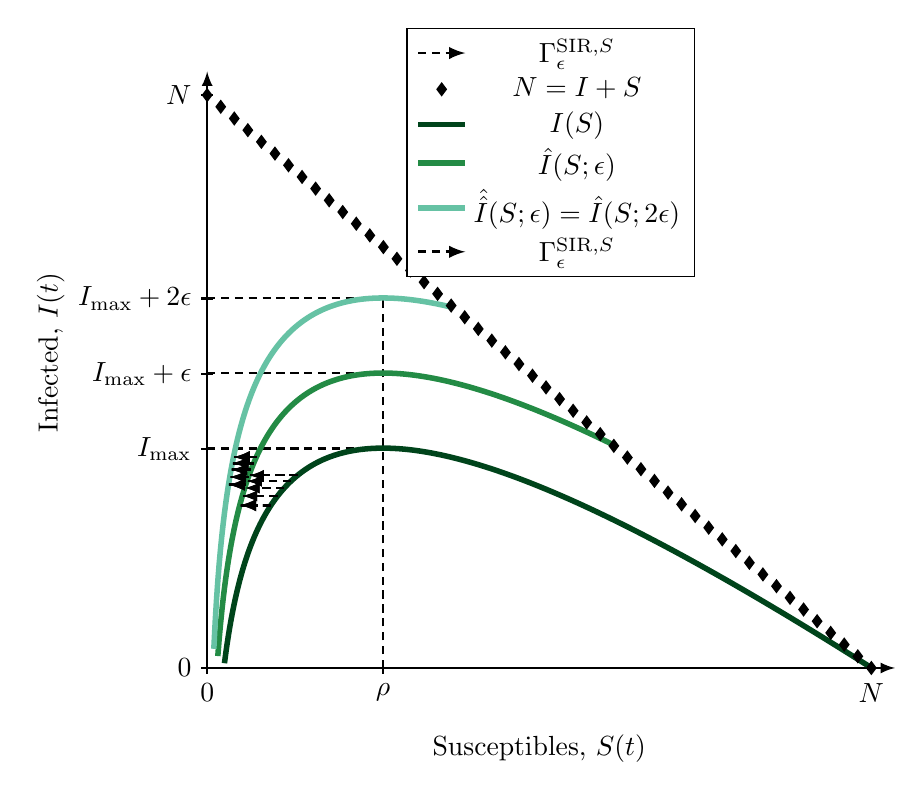
\begin{tikzpicture}
  % The axis of the plot
\begin{axis}[
    xlabel={Susceptibles, $S(t)$},
    ylabel={Infected, $I(t)$},
    x label style={at={(axis description cs:0.5,-0.1)},anchor=north},
    y label style={at={(axis description cs:-0.2,0.55)},rotate=90,anchor=south},
    scaled x ticks = false,
    legend style={at={(axis description cs:0.3,0.9)},anchor=west,nodes={scale=1.00, transform shape}},    
    grid style=dashed,
    extra x ticks = {0},
    extra y ticks= {0},    
    xticklabels={$0$, $\rho$, $N$},
    xtick={0,202,763},
    yticklabels={$0$, $I_{\max}$,$I_{\max}+\epsilon$,$I_{\max}+2\epsilon$, $N$},
    ytick={0,292,392,492,763}, ]
    ]
    
\addplot[
color=black,->,>=latex,densely dashed,line width=1.0pt
]
coordinates {%
(73.29859719438878,216.73757566719837)
(72.17324734947816,216.73757566719837)
(71.07455327246905,216.73757566719837)
(70.00145359533154,216.73757566719837)
(68.95295183975871,216.73757566719837)
(67.92811102562075,216.73757566719837)
(66.92604884127269,216.73757566719837)
(65.94593330581621,216.73757566719837)
(64.98697886345734,216.73757566719837)
(64.04844285854115,216.73757566719837)
(63.12962234687957,216.7375756671984)
(62.22985120502502,216.73757566719837)
(61.34849750416434,216.73757566719834)
(60.48496111964311,216.73757566719837)
(59.63867155080259,216.7375756671984)
(58.809085928965374,216.73757566719837)
(57.99568719411242,216.73757566719837)
(57.19798242312862,216.73757566719837)
(56.41550129450782,216.73757566719837)
(55.647794676158554,216.73757566719837)
(54.89443332446261,216.73757566719837)
(54.15500668408743,216.7375756671984)
(53.42912177914677,216.73757566719837)
(52.71640218740301,216.73757566719837)
(52.016487090013904,216.73757566719837)
(51.32903039014982,216.73757566719834)
(50.653699894481704,216.73757566719837)
(49.990176552148476,216.73757566719837)
(49.33815374635204,216.73757566719837)
(48.6973366342027,216.7375756671984)
(48.06744153086277,216.73757566719837)
(47.4481953344118,216.73757566719837)
(46.839334988193414,216.73757566719837)
(46.24060697770488,216.73757566719837)
(45.6517668593568,216.73757566719837)
(45.0725788186767,216.73757566719837)
(44.502815255724244,216.73757566719837)
(43.942256395733295,216.73757566719837)
(43.39068992309406,216.73757566719834)
(42.84791063701392,216.73757566719837)
(42.313720127301174,216.7375756671984)
(41.787926468856085,216.73757566719837)
(41.270343933567474,216.73757566719837)
(40.76079271842093,216.7375756671984)
(40.25909868871557,216.73757566719837)
(39.76509313537706,216.73757566719837)
(39.278612545450635,216.73757566719834)
(38.79949838486956,216.73757566719837)
(38.32759689275532,216.73757566719837)
(37.86275888647898,216.73757566719837)
};
\addlegendentry{$\Gamma^{\mathrm{SIR},S}_{\epsilon}$}
\addplot[
forget plot,
color=black,->,>=latex,densely dashed
]
coordinates {%
(80.93386773547094,229.11866746025078)
(79.61497606877097,229.11866746025078)
(78.33118829125114,229.11866746025078)
(77.08087330528886,229.11866746025078)
(75.86251713720564,229.1186674602508)
(74.67471154120578,229.11866746025078)
(73.51614398885384,229.11866746025075)
(72.38558884371298,229.11866746025078)
(71.28189955411469,229.11866746025078)
(70.20400172422309,229.1186674602508)
(69.15088694553633,229.11866746025078)
(68.12160728941313,229.11866746025078)
(67.11527037604705,229.11866746025078)
(66.1310349478865,229.11866746025075)
(65.16810688586524,229.11866746025078)
(64.22573561551619,229.11866746025078)
(63.30321085735364,229.11866746025078)
(62.399859682085484,229.11866746025078)
(61.51504383643975,229.11866746025078)
(60.648157309857915,229.1186674602508)
(59.79862411604493,229.11866746025078)
(58.96589626668804,229.11866746025078)
(58.149451917376794,229.1186674602508)
(57.348793668189785,229.11866746025078)
(56.56344700347902,229.11866746025078)
(55.792958857175435,229.11866746025078)
(55.036896291501684,229.11866746025078)
(54.294845278332794,229.11866746025075)
(53.566409573633216,229.11866746025078)
(52.85120967643358,229.11866746025078)
(52.14888186472073,229.11866746025078)
(51.459077301414524,229.11866746025078)
(50.78146120431264,229.11866746025078)
(50.115712074486,229.11866746025078)
(49.46152097820823,229.11866746025078)
(48.81859087791802,229.11866746025078)
(48.18663600821013,229.11866746025078)
(47.565381293200446,229.11866746025078)
(46.95456180196698,229.11866746025075)
(46.35392223907112,229.1186674602508)
(45.76321646743891,229.11866746025078)
(45.18220706112643,229.11866746025078)
(44.6106648857257,229.11866746025078)
(44.04836870433148,229.11866746025078)
(43.49510480721821,229.11866746025075)
(42.950666663492875,229.1186674602508)
(42.41485459315706,229.11866746025078)
(41.887475458137104,229.11866746025078)
(41.36834237095959,229.11866746025078)
(40.857274419857426,229.11866746025078)
};
\addplot[
forget plot,
color=black,->,>=latex,densely dashed
]
coordinates {%
(88.5691382765531,239.6939185120168)
(87.03154398094865,239.6939185120168)
(85.54024532058186,239.6939185120168)
(84.09272202410762,239.6939185120168)
(82.68666663626615,239.6939185120168)
(81.31996026397695,239.6939185120168)
(79.99065176119576,239.6939185120168)
(78.69693977502212,239.6939185120168)
(77.43715718682064,239.6939185120168)
(76.20975756918646,239.6939185120168)
(75.01330334868126,239.6939185120168)
(73.84645541896808,239.6939185120168)
(72.70796399301364,239.6939185120168)
(71.59666051844816,239.6939185120168)
(70.51145050894611,239.6939185120168)
(69.45130716795292,239.6939185120168)
(68.41526570034826,239.6939185120168)
(67.40241822349007,239.6939185120168)
(66.41190920230842,239.69391851201678)
(65.4429313439174,239.6939185120168)
(64.4947218965766,239.69391851201684)
(63.566559305342416,239.6939185120168)
(62.65776018332185,239.69391851201678)
(61.76767656289773,239.6939185120168)
(60.89569339595266,239.69391851201684)
(60.04122627608874,239.6939185120168)
(59.20371935922963,239.69391851201678)
(58.38264346190641,239.6939185120168)
(57.57749431902922,239.69391851201684)
(56.78779098511216,239.6939185120168)
(56.01307436477417,239.69391851201678)
(55.25290585999997,239.6939185120168)
(54.50686612300195,239.6939185120168)
(53.774553904804264,239.6939185120168)
(53.05558499072296,239.6939185120168)
(52.3495912148666,239.6939185120168)
(51.65621954661149,239.6939185120168)
(50.97513124273385,239.69391851201678)
(50.30600105952632,239.6939185120168)
(49.648516519812176,239.6939185120168)
(49.00237723022441,239.6939185120168)
(48.367294244642466,239.69391851201684)
(47.74298947000781,239.6939185120168)
(47.129195111132745,239.6939185120168)
(46.525653151422055,239.6939185120168)
(45.932114866710336,239.69391851201678)
(45.34834036967377,239.6939185120168)
(44.7740981825012,239.6939185120168)
(44.20916483571146,239.6939185120168)
(43.65332449119373,239.69391851201684)
};
\addplot[
forget plot,
color=black,->,>=latex,densely dashed
]
coordinates {%
(96.20440881763527,248.76237457164757)
(94.41779706104012,248.76237457164757)
(92.69249242235995,248.76237457164757)
(91.02456660880688,248.76237457164757)
(89.41048219645084,248.76237457164757)
(87.84704040476382,248.76237457164757)
(86.33133750718366,248.76237457164757)
(84.86072819457226,248.76237457164757)
(83.43279458276626,248.76237457164754)
(82.04531983700268,248.76237457164757)
(80.6962655997855,248.7623745716476)
(79.38375257288544,248.76237457164757)
(78.10604373119898,248.76237457164754)
(76.86152974539499,248.76237457164757)
(75.64871626835499,248.7623745716476)
(74.46621280231996,248.76237457164757)
(73.31272291313596,248.76237457164757)
(72.18703559761977,248.76237457164754)
(71.08801764235842,248.76237457164757)
(70.01460683826791,248.76237457164757)
(68.96580593669626,248.76237457164757)
(67.94067725042517,248.7623745716476)
(66.9383378174609,248.76237457164757)
(65.95795505758112,248.76237457164757)
(64.99874286166964,248.76237457164757)
(64.05995806230744,248.76237457164754)
(63.14089724118503,248.76237457164757)
(62.240893834898166,248.76237457164757)
(61.35931550572795,248.76237457164757)
(60.495561748427555,248.7623745716476)
(59.649061707581815,248.76237457164757)
(58.81927218338574,248.76237457164757)
(58.00567580634005,248.7623745716476)
(57.20777936371328,248.76237457164757)
(56.425112262640724,248.76237457164757)
(55.657225116472304,248.76237457164754)
(54.90368844253971,248.76237457164757)
(54.16409146074857,248.76237457164757)
(53.43804098368304,248.76237457164754)
(52.725160389816445,248.76237457164757)
(52.025088672365584,248.7623745716476)
(51.33747955709161,248.76237457164757)
(50.66200068304288,248.76237457164757)
(49.9983328408407,248.7623745716476)
(49.34616926364862,248.76237457164757)
(48.70521496644559,248.76237457164757)
(48.07518612964232,248.76237457164754)
(47.455809523462186,248.76237457164757)
(46.84682196984221,248.76237457164757)
(46.247969838911565,248.76237457164757)
};
\addplot[
forget plot,
color=black,->,>=latex,densely dashed
]
coordinates {%
(103.83967935871743,256.5544457450492)
(101.76710245838181,256.5544457450492)
(99.77625373509215,256.5544457450492)
(97.86093693300178,256.5544457450492)
(96.01568423806941,256.5544457450492)
(94.23564200280197,256.5544457450492)
(92.5164785210507,256.5544457450492)
(90.85430886700026,256.5544457450492)
(89.24563309232168,256.5544457450492)
(87.68728499051676,256.5544457450492)
(86.17638930141702,256.5544457450492)
(84.71032571689548,256.5544457450492)
(83.28669841212529,256.5544457450492)
(81.9033101001365,256.5544457450492)
(80.55813981541678,256.5544457450492)
(79.24932379194225,256.5544457450492)
(77.9751389248944,256.5544457450492)
(76.7339884019646,256.5544457450492)
(75.5243891663796,256.5544457450492)
(74.34496093423385,256.5544457450492)
(73.19441653702793,256.5544457450492)
(72.07155339917092,256.5544457450492)
(70.97524599165203,256.5544457450492)
(69.90443912868723,256.5544457450492)
(68.85814199510418,256.5544457450492)
(67.83542280943794,256.5544457450492)
(66.83540404204324,256.5544457450492)
(65.85725811926257,256.5544457450492)
(64.9002035546684,256.5544457450492)
(63.96350145663152,256.5544457450492)
(63.04645236845014,256.5544457450492)
(62.148393403166125,256.5544457450492)
(61.268695640171075,256.5544457450492)
(60.40676175501495,256.5544457450492)
(59.56202385731988,256.5544457450492)
(58.733941514999266,256.5544457450492)
(57.921999945489304,256.5544457450492)
(57.125708357089295,256.5544457450492)
(56.34459842546975,256.5544457450492)
(55.5782228921383,256.5544457450492)
(54.82615427313491,256.5544457450492)
(54.08798366759356,256.5544457450492)
(53.363319656830456,256.5544457450492)
(52.65178728576548,256.5544457450492)
(51.95302711924113,256.5544457450492)
(51.26669436663699,256.5544457450492)
(50.59245806883385,256.5544457450492)
(49.93000034219901,256.5544457450492)
(49.27901567476974,256.5544457450492)
(48.63921027031561,256.5544457450492)
};
\addplot[
forget plot,
color=black,->,>=latex,densely dashed,line width=1.0pt
]
coordinates {%
(44.28456913827655,243.96275717718436)
(43.72751880816169,243.96275717718436)
(43.1793805426799,243.96275717718436)
(42.639951809196475,243.96275717718436)
(42.10903674517267,243.96275717718436)
(41.586445859551574,243.96275717718436)
(41.07199575106974,243.96275717718436)
(40.56550884234436,243.96275717718436)
(40.066813128668784,243.96275717718436)
(39.57574194053553,243.96275717718436)
(39.09213371898182,243.96275717718436)
(38.61583180292274,243.96275717718436)
(38.14668422769545,243.96275717718436)
(37.68454353412256,243.96275717718436)
(37.22926658738978,243.96275717718436)
(36.78071440517542,243.96275717718436)
(36.33875199443153,243.96275717718436)
(35.903248196301774,243.96275717718436)
(35.47407553868386,243.96275717718436)
(35.05111009598265,243.96275717718436)
(34.63423135562951,243.96275717718436)
(34.22332209097404,243.96275717718436)
(33.81826824018095,243.96275717718436)
(33.4189587907889,243.96275717718436)
(33.02528566961169,243.96275717718436)
(32.63714363768329,243.96275717718436)
(32.25443018996736,243.96275717718436)
(31.877045459569818,243.96275717718436)
(31.504892126207256,243.96275717718436)
(31.137875328718888,243.96275717718436)
(30.775902581370957,243.96275717718436)
(30.418883693795863,243.96275717718436)
(30.06673069434747,243.96275717718436)
(29.719357756707122,243.96275717718436)
(29.376681129570972,243.96275717718436)
(29.038619069263127,243.96275717718436)
(28.705091775126775,243.96275717718436)
(28.37602132755504,243.96275717718436)
(28.05133162853094,243.96275717718436)
(27.73094834455367,243.96275717718436)
(27.41479885183528,243.96275717718436)
(27.102812183658475,243.96275717718436)
(26.794918979792133,243.96275717718436)
(26.491051437867903,243.96275717718436)
(26.19114326662492,243.96275717718436)
(25.895129640936588,243.96275717718436)
(25.60294715853825,243.96275717718436)
(25.314533798370157,243.96275717718436)
(25.029828880479872,243.96275717718436)
(24.748773027393064,243.96275717718436)
};
\addplot[
forget plot,
color=black,->,>=latex,densely dashed,line width=1.0pt
]
coordinates {%
(47.33867735470942,254.38030660948323)
(46.73164532441587,254.38030660948323)
(46.13470131143206,254.38030660948323)
(45.54760244522679,254.38030660948323)
(44.97011440838551,254.38030660948323)
(44.402011026686196,254.38030660948323)
(43.84307388402975,254.38030660948323)
(43.29309196042041,254.38030660948323)
(42.75186129132952,254.38030660948323)
(42.21918464692141,254.38030660948323)
(41.69487122974633,254.38030660948323)
(41.17873638961531,254.38030660948323)
(40.670601354490934,254.38030660948323)
(40.17029297628901,254.38030660948323)
(39.67764349061623,254.38030660948323)
(39.1924902895091,254.38030660948323)
(38.714675706330056,254.38030660948323)
(38.24404681203551,254.38030660948323)
(37.78045522209023,254.38030660948323)
(37.32375691335716,254.38030660948323)
(36.87381205034036,254.38030660948323)
(36.43048482020451,254.38030660948323)
(35.99364327603572,254.38030660948323)
(35.56315918784715,254.38030660948323)
(35.13890790086648,254.38030660948323)
(34.720768200676304,254.38030660948323)
(34.30862218480677,254.38030660948323)
(33.90235514040476,254.38030660948323)
(33.50185542764716,254.38030660948323)
(33.10701436854041,254.38030660948323)
(32.717726140842885,254.38030660948323)
(32.333887676800344,254.38030660948323)
(31.955398566438912,254.38030660948323)
(31.58216096516726,254.38030660948323)
(31.214079505454905,254.38030660948323)
(30.851061212370016,254.38030660948323)
(30.493015422772373,254.38030660948323)
(30.139853707970385,254.38030660948323)
(29.791489799662806,254.38030660948323)
(29.44783951899602,254.38030660948323)
(29.108820708578804,254.38030660948323)
(28.77435316730522,254.38030660948323)
(28.444358587845276,254.38030660948323)
(28.11876049667164,254.38030660948323)
(27.79748419649727,254.38030660948323)
(27.480456711009545,254.38030660948323)
(27.167606731779124,254.38030660948323)
(26.858864567262042,254.38030660948323)
(26.554162093770195,254.38030660948323)
(26.25343270833426,254.38030660948323)
};
\addplot[
forget plot,
color=black,->,>=latex,densely dashed,line width=1.0pt
]
coordinates {%
(50.392785571142284,263.95531050327986)
(49.73379630914956,263.95531050327986)
(49.08619089401573,263.95531050327986)
(48.44967891813922,263.95531050327986)
(47.82398090234941,263.95531050327986)
(47.20882773580733,263.95531050327986)
(46.60396015219504,263.95531050327986)
(46.00912823937501,263.95531050327986)
(45.42409097994233,263.95531050327986)
(44.84861582032584,263.95531050327986)
(44.28247826630298,263.95531050327986)
(43.7254615029726,263.95531050327986)
(43.17735603742332,263.95531050327986)
(42.637959362429,263.95531050327986)
(42.107075639718076,263.95531050327986)
(41.58451540142,263.95531050327986)
(41.070095268439225,263.95531050327986)
(40.56363768459906,263.95531050327986)
(40.064970665489895,263.95531050327986)
(39.57392756104138,263.95531050327986)
(39.090346830914214,263.95531050327986)
(38.614071831876316,263.95531050327986)
(38.1449506163917,263.95531050327986)
(37.68283574170963,263.95531050327986)
(37.22758408879201,263.95531050327986)
(36.779056690468266,263.95531050327986)
(36.33711856824671,263.95531050327986)
(35.90163857727019,263.95531050327986)
(35.47248925889586,263.95531050327986)
(35.049546700479844,263.95531050327986)
(34.632690401920044,263.95531050327986)
(34.22180314857073,263.95531050327986)
(33.81677089016112,263.95531050327986)
(33.417482625374774,263.95531050327986)
(33.023830291770025,263.95531050327986)
(32.635708660743354,263.95531050327986)
(32.25301523725575,263.95531050327986)
(31.87565016406213,263.95531050327986)
(31.503516130197948,263.95531050327986)
(31.13651828349579,263.95531050327986)
(30.774564146916237,263.95531050327986)
(30.417563538492697,263.95531050327986)
(30.06542849470099,263.95531050327986)
(29.718073197076627,263.95531050327986)
(29.375413901916495,263.95531050327986)
(29.03736887289419,263.95531050327986)
(28.703858316471216,263.95531050327986)
(28.374804319931844,263.95531050327986)
(28.050130791933448,263.95531050327986)
(27.72976340544131,263.95531050327986)
};
\addplot[
forget plot,
color=black,->,>=latex,densely dashed,line width=1.0pt
]
coordinates {%
(53.44689378757515,272.7869832914795)
(52.73385337146748,272.7869832914795)
(52.033626182467415,272.7869832914795)
(51.3458657701663,272.7869832914795)
(50.670239607156674,272.7869832914795)
(50.00642832665072,272.7869832914795)
(49.35412501282452,272.7869832914795)
(48.713034539521814,272.7869832914795)
(48.08287295334779,272.7869832914795)
(47.46336689756877,272.7869832914795)
(46.85425307356814,272.7869832914795)
(46.255277736920334,272.7869832914795)
(45.66619622538834,272.7869832914795)
(45.086772516426755,272.7869832914795)
(44.516778811959,272.7869832914795)
(43.955995148407915,272.7869832914795)
(43.404209030128214,272.7869832914795)
(42.86121508454965,272.7869832914795)
(42.326814737481506,272.7869832914795)
(41.80081590715735,272.7869832914795)
(41.2830327157166,272.7869832914795)
(40.773285216925196,272.7869832914795)
(40.27139913903298,272.7869832914795)
(39.77720564175296,272.7869832914795)
(39.290541086427645,272.7869832914795)
(38.81124681851612,272.7869832914795)
(38.33916896161831,272.7869832914795)
(37.87415822227081,272.7869832914795)
(37.416069704865954,272.7869832914795)
(36.964762736039624,272.7869832914795)
(36.52010069795081,272.7869832914795)
(36.08195086990822,272.7869832914795)
(35.650184277839394,272.7869832914795)
(35.2246755511335,272.7869832914795)
(34.80530278642146,272.7869832914795)
(34.391947417887636,272.7869832914795)
(33.984494093734796,272.7869832914795)
(33.58283055844954,272.7869832914795)
(33.186847540539155,272.7869832914795)
(32.796438645433035,272.7869832914795)
(32.41150025326108,272.7869832914795)
(32.031931421241055,272.7869832914795)
(31.65763379042355,272.7869832914795)
(31.288511496563043,272.7869832914795)
(30.924471084877567,272.7869832914795)
(30.565421428526907,272.7869832914795)
(30.21127365057302,272.7869832914795)
(29.861941049269355,272.7869832914795)
(29.517339026497876,272.7869832914795)
(29.177385019194766,272.7869832914795)
};
\addplot[
forget plot,
color=black,->,>=latex,densely dashed,line width=1.0pt
]
coordinates {%
(56.501002004008015,280.95798500831836)
(55.731688561577606,280.95798500831836)
(54.97676675320878,280.95798500831836)
(54.235824019981884,280.95798500831836)
(53.50846550040466,280.95798500831836)
(52.794312995853204,280.95798500831836)
(52.09300401232809,280.95798500831836)
(51.40419087178919,280.95798500831836)
(50.72753988698955,280.95798500831836)
(50.06273059435584,280.95798500831836)
(49.40945504000327,280.95798500831836)
(48.76741711447241,280.95798500831836)
(48.136331932163706,280.95798500831836)
(47.5159252518847,280.95798500831836)
(46.90593293521441,280.95798500831836)
(46.3061004397218,280.95798500831836)
(45.716182344336566,280.95798500831836)
(45.13594190441718,280.95798500831836)
(44.565150634278226,280.95798500831836)
(44.00358791513616,280.95798500831836)
(43.45104062660961,280.95798500831836)
(42.90730280006875,280.95798500831836)
(42.37217529227294,280.95798500831836)
(41.8454654778661,280.95798500831836)
(41.32698695941314,280.95798500831836)
(40.81655929378361,280.95798500831836)
(40.31400773374719,280.95798500831836)
(39.819162983787905,280.95798500831836)
(39.33186096917667,280.95798500831836)
(38.85194261743929,280.95798500831836)
(38.379253651416875,280.95798500831836)
(37.91364439317648,280.95798500831836)
(37.45496957808561,280.95798500831836)
(37.00308817841461,280.95798500831836)
(36.55786323587792,280.95798500831836)
(36.11916170256738,280.95798500831836)
(35.686854289769435,280.95798500831836)
(35.260815324194986,280.95798500831836)
(34.84092261118269,280.95798500831836)
(34.42705730446747,280.95798500831836)
(34.01910378213322,280.95798500831836)
(33.616949528397285,280.95798500831836)
(33.22048502088674,280.95798500831836)
(32.82960362311599,280.95798500831836)
(32.444201481855345,280.95798500831836)
(32.06417742913517,280.95798500831836)
(31.689432888627902,280.95798500831836)
(31.319871786171834,280.95798500831836)
(30.955400464215746,280.95798500831836)
(30.595927599976307,280.95798500831836)
};
\addplot[
color=black,mark=diamond*,only marks,line width=0.75pt,
]
coordinates {%
(0.0,763.0)
(15.57142857142857,747.4285714285714)
(31.14285714285714,731.8571428571428)
(46.714285714285715,716.2857142857143)
(62.28571428571428,700.7142857142858)
(77.85714285714285,685.1428571428571)
(93.42857142857143,669.5714285714286)
(109.0,654.0)
(124.57142857142856,638.4285714285714)
(140.14285714285714,622.8571428571429)
(155.7142857142857,607.2857142857143)
(171.28571428571428,591.7142857142857)
(186.85714285714286,576.1428571428571)
(202.4285714285714,560.5714285714286)
(218.0,545.0)
(233.57142857142853,529.4285714285716)
(249.1428571428571,513.8571428571429)
(264.7142857142857,498.28571428571433)
(280.2857142857143,482.7142857142857)
(295.85714285714283,467.14285714285717)
(311.4285714285714,451.57142857142856)
(327.0,436.0)
(342.57142857142856,420.42857142857144)
(358.1428571428571,404.8571428571429)
(373.7142857142857,389.2857142857143)
(389.2857142857143,373.7142857142857)
(404.8571428571428,358.1428571428572)
(420.4285714285714,342.5714285714286)
(436.0,327.0)
(451.57142857142856,311.42857142857144)
(467.14285714285705,295.85714285714295)
(482.71428571428567,280.28571428571433)
(498.2857142857142,264.7142857142858)
(513.8571428571429,249.14285714285717)
(529.4285714285714,233.57142857142858)
(544.9999999999999,218.00000000000009)
(560.5714285714286,202.42857142857147)
(576.1428571428571,186.8571428571429)
(591.7142857142857,171.2857142857143)
(607.2857142857142,155.7142857142858)
(622.8571428571428,140.14285714285722)
(638.4285714285713,124.57142857142863)
(654.0,109.00000000000004)
(669.5714285714286,93.42857142857144)
(685.1428571428571,77.85714285714295)
(700.7142857142857,62.285714285714356)
(716.2857142857142,46.714285714285765)
(731.8571428571428,31.142857142857178)
(747.4285714285714,15.571428571428589)
(763.0,0.0)
};
\addlegendentry{$N=I+S$}
\addplot[
forget plot,
color=black,densely dashed,line width=1.0pt,
]
coordinates {%
(0,292.8088706263408)
(202,292.8088706263408)
};
\addplot[
forget plot,
color=black,densely dashed,line width=1.0pt,
]
coordinates {%
(0,392.8088706263408)
(202,392.8088706263408)
};
\addplot[
forget plot,
color=black,densely dashed,line width=1.0pt,
]
coordinates {%
(0,492.8088706263408)
(202,492.8088706263408)
};
\addplot[
forget plot,
color=black,densely dashed,line width=1.0pt,
]
coordinates {%
(202,0)
(202,492.8088706263408)
};
\addplot[
color=clr_1,line width=2.0pt,
]
coordinates {%
(19.851703406813627,6.321635458609876)
(21.37875751503006,19.764391725445307)
(22.905811623246493,32.1738976575931)
(24.432865731462925,43.683624819166084)
(25.95991983967936,54.402744317869406)
(27.48697394789579,64.42168980532267)
(29.014028056112224,73.8162143937019)
(30.541082164328657,82.65040575177068)
(32.06813627254509,90.97896480577947)
(33.59519038076152,98.84895385581137)
(35.122244488977955,106.30115578690345)
(36.64929859719439,113.37114379128377)
(38.17635270541082,120.0901325761588)
(39.703406813627254,126.48566252490525)
(41.23046092184369,132.58215466922388)
(42.75751503006012,138.4013646835242)
(44.28456913827655,143.96275717718436)
(45.811623246492985,149.28381650745553)
(47.33867735470942,154.38030660948323)
(48.86573146292585,159.26648956081203)
(50.392785571142284,163.95531050327986)
(51.91983967935872,168.458554951299)
(53.44689378757515,172.7869832914795)
(54.97394789579158,176.9504463305359)
(56.501002004008015,180.95798500831836)
(58.02805611222445,184.81791681069865)
(59.55511022044088,188.5379109559409)
(61.08216432865731,192.12505406055095)
(62.609218436873746,195.58590769558964)
(64.13627254509018,198.92655900634338)
(65.66332665330661,202.1526653749861)
(67.19038076152304,205.2694939481587)
(68.71743486973948,208.28195672205823)
(70.24448897795591,211.1946417710344)
(71.77154308617234,214.01184111745272)
(73.29859719438878,216.73757566719837)
(74.82565130260521,219.3756175739344)
(76.35270541082164,221.92951034385692)
(77.87975951903807,224.40258694946874)
(79.40681362725451,226.797986184387)
(80.93386773547094,229.11866746025078)
(82.46092184368737,231.36742422048928)
(83.9879759519038,233.54689612324842)
(85.51503006012024,235.65958012657302)
(87.04208416833667,237.70784059243556)
(88.5691382765531,239.6939185120168)
(90.09619238476954,241.61993994237878)
(91.62324649298597,243.4879237340714)
(93.1503006012024,245.29978861999973)
(94.67735470941884,247.05735972788284)
(96.20440881763527,248.76237457164757)
(97.7314629258517,250.41648857099517)
(99.25851703406813,252.02128014304367)
(100.78557114228457,253.57825540524652)
(102.312625250501,255.08885252466723)
(103.83967935871743,256.5544457450492)
(105.36673346693387,257.97634911990565)
(106.8937875751503,259.3558199770133)
(108.42084168336673,260.6940621371722)
(109.94789579158316,261.99222890785313)
(111.4749498997996,263.2514258703685)
(113.00200400801603,264.47271347741935)
(114.52905811623246,265.6571094762953)
(116.0561122244489,266.80559117158305)
(117.58316633266533,267.91909753997186)
(119.11022044088176,268.99853120860894)
(120.6372745490982,270.0447603074334)
(122.16432865731463,271.0586202050025)
(123.69138276553106,272.0409151364946)
(125.21843687374749,272.9924197318247)
(126.74549098196393,273.91388045114195)
(128.27254509018036,274.8060169343622)
(129.79959919839678,275.66952327084016)
(131.32665330661322,276.50506919478835)
(132.85370741482967,277.3133012115894)
(134.3807615230461,278.0948436597447)
(135.9078156312625,278.8502997128228)
(137.43486973947896,279.58025232542775)
(138.9619238476954,280.28526512690144)
(140.48897795591182,280.96588326618746)
(142.01603206412824,281.6226342110225)
(143.5430861723447,282.2560285043892)
(145.07014028056113,282.8665604809412)
(146.59719438877755,283.45470894591847)
(148.12424849699397,284.02093781888254)
(149.65130260521042,284.56569674443824)
(151.17835671342687,285.08942167195346)
(152.70541082164328,285.5925354061443)
(154.2324649298597,286.0754481302678)
(155.75951903807615,286.53855790353964)
(157.2865731462926,286.982251134287)
(158.81362725450902,287.40690303024144)
(160.34068136272543,287.8128780272873)
(161.86773547094188,288.20053019788884)
(163.39478957915833,288.57020364033986)
(164.92184368737475,288.92223284991064)
(166.44889779559117,289.25694307288904)
(167.9759519038076,289.5746506444535)
(169.50300601202406,289.8756633112605)
(171.03006012024048,290.16028053956165)
(172.5571142284569,290.42879380962904)
(174.08416833667334,290.68148689720795)
(175.6112224448898,290.9186361426798)
(177.1382765531062,291.1405107085727)
(178.66533066132263,291.34737282601725)
(180.19238476953907,291.5394780307183)
(181.71943887775552,291.7170753889668)
(183.24649298597194,291.8804077141946)
(184.77354709418836,292.0297117745463)
(186.3006012024048,292.1652184919062)
(187.82765531062125,292.2871531328002)
(189.35470941883767,292.39573549157285)
(190.8817635270541,292.4911800662039)
(192.40881763527054,292.5736962271211)
(193.93587174348698,292.64348837934153)
(195.4629258517034,292.70075611825246)
(196.98997995991982,292.7456943793311)
(198.51703406813627,292.7784935820845)
(200.04408817635272,292.7993397684729)
(201.57114228456913,292.808414736071)
(203.09819639278555,292.80589616620193)
(204.625250501002,292.7919577472751)
(206.15230460921845,292.76676929353766)
(207.67935871743487,292.7304968594407)
(209.20641282565128,292.6833028498229)
(210.73346693386773,292.6253461260808)
(212.26052104208418,292.5567821085086)
(213.7875751503006,292.47776287497186)
(215.31462925851702,292.388437256066)
(216.84168336673346,292.2889509269145)
(218.3687374749499,292.1794464957445)
(219.89579158316633,292.06006358937907)
(221.42284569138275,291.93093893576656)
(222.9498997995992,291.79220644367786)
(224.47695390781564,291.64399727968225)
(226.00400801603206,291.48643994251233)
(227.53106212424848,291.31966033492756)
(229.05811623246493,291.14378183317194)
(230.58517034068137,290.9589253541267)
(232.1122244488978,290.7652094202432)
(233.6392785571142,290.5627502223508)
(235.16633266533066,290.3516616804154)
(236.6933867735471,290.13205550233386)
(238.22044088176352,289.904041240836)
(239.74749498997994,289.6677263485715)
(241.2745490981964,289.42321623144414)
(242.80160320641284,289.17061430026706)
(244.32865731462925,288.910022020797)
(245.85571142284567,288.6415389622091)
(247.38276553106212,288.3652628440726)
(248.90981963927857,288.0812895818806)
(250.43687374749499,287.78971333118625)
(251.9639278557114,287.490626530399)
(253.49098196392785,287.184119942287)
(255.0180360721443,286.8702826942333)
(256.5450901803607,286.5492023172907)
(258.07214428857714,286.22096478407684)
(259.59919839679355,285.88565454555237)
(261.12625250501003,285.54335456672027)
(262.65330661322645,285.1941463612841)
(264.18036072144287,284.8381100253016)
(265.70741482965934,284.4753242698688)
(267.23446893787576,284.1058664528671)
(268.7615230460922,283.7298126098076)
(270.2885771543086,283.34723748379815)
(271.815631262525,282.9582145546693)
(273.3426853707415,282.5628160672841)
(274.8697394789579,282.1611130590579)
(276.39679358717433,281.7531753867155)
(277.9238476953908,281.339071752315)
(279.4509018036072,280.91886972855286)
(280.97795591182364,280.49263578338457)
(282.50501002004006,280.0604353039746)
(284.0320641282565,279.62233262000336)
(285.55911823647295,279.17839102634673)
(287.0861723446894,278.72867280515356)
(288.6132264529058,278.2732392473349)
(290.14028056112227,277.8121506734891)
(291.6673346693387,277.3454664542737)
(293.1943887775551,276.87324503025)
(294.7214428857715,276.3955439312085)
(296.24849699398794,275.9124197949976)
(297.7755511022044,275.42392838586557)
(299.30260521042084,274.93012461233684)
(300.82965931863725,274.4310625446295)
(302.35671342685373,273.9267954316356)
(303.88376753507015,273.4173757174706)
(305.41082164328657,272.90285505761005)
(306.937875751503,272.38328433462334)
(308.4649298597194,271.85871367351706)
(309.9919839679359,271.32919245669825)
(311.5190380761523,270.79476933857245)
(313.0460921843687,270.25549225978284)
(314.5731462925852,269.71140846110336)
(316.1002004008016,269.1625644969961)
(317.62725450901803,268.6090062488413)
(319.15430861723445,268.0507789378505)
(320.68136272545087,267.4879271376709)
(322.20841683366734,266.9204947866913)
(323.73547094188376,266.348525200056)
(325.2625250501002,265.7720610813968)
(326.78957915831666,265.1911445342905)
(328.3166332665331,264.60581707344795)
(329.8436873747495,264.01611963564494)
(331.3707414829659,263.4220925904001)
(332.89779559118233,262.82377575040687)
(334.4248496993988,262.2212083817275)
(335.9519038076152,261.6144292137549)
(337.47895791583164,261.0034764489476)
(339.0060120240481,260.3883877723455)
(340.53306613226454,259.7692003608727)
(342.06012024048096,259.14595089243016)
(343.5871743486974,258.5186755547886)
(345.1142284569138,257.8874100542811)
(346.64128256513027,257.2521896243063)
(348.1683366733467,256.6130490336434)
(349.6953907815631,255.97002259458634)
(351.2224448897796,255.323144170899)
(352.749498997996,254.67244718559937)
(354.2765531062124,254.01796462857544)
(355.80360721442884,253.35972906403572)
(357.33066132264526,252.69777263780338)
(358.85771543086173,252.03212708445164)
(360.38476953907815,251.3628237342882)
(361.91182364729457,250.68989352019503)
(363.43887775551104,250.01336698432)
(364.96593186372746,249.33327428463076)
(366.4929859719439,248.64964520133162)
(368.0200400801603,247.9625091431451)
(369.5470941883767,247.27189515346697)
(371.0741482965932,246.57783191639078)
(372.6012024048096,245.8803477626102)
(374.12825651302603,245.17947067520197)
(375.6553106212425,244.47522829528793)
(377.1823647294589,243.7676479275858)
(378.70941883767534,243.056756545844)
(380.23647294589176,242.34258079817232)
(381.7635270541082,241.6251470122586)
(383.29058116232466,240.9044812004887)
(384.8176352705411,240.18060906495953)
(386.3446893787575,239.45355600239486)
(387.87174348697397,238.7233471089636)
(389.3987975951904,237.99000718500474)
(390.9258517034068,237.25356073965804)
(392.4529058116232,236.51403199540437)
(393.97995991983964,235.7714448925202)
(395.5070140280561,235.0258230934437)
(397.03406813627254,234.27718998705723)
(398.56112224448896,233.5255686928882)
(400.08817635270543,232.7709820652292)
(401.61523046092185,232.0134526971799)
(403.14228456913827,231.25300292461077)
(404.6693386773547,230.48965483005531)
(406.1963927855711,229.72343024652537)
(407.7234468937876,228.95435076125602)
(409.250501002004,228.18243771938205)
(410.7775551102204,227.40771222754415)
(412.3046092184369,226.63019515742815)
(413.8316633266533,225.84990714923947)
(415.35871743486973,225.0668686151148)
(416.88577154308615,224.281099742469)
(418.41282565130257,223.49262049728065)
(419.93987975951904,222.7014506273215)
(421.46693386773546,221.90760966532207)
(422.9939879759519,221.11111693208375)
(424.52104208416836,220.31199153953344)
(426.0480961923848,219.51025239372416)
(427.5751503006012,218.7059181977803)
(429.1022044088176,217.89900745479213)
(430.62925851703403,217.089538470658)
(432.1563126252505,216.2775293568767)
(433.6833667334669,215.46299803328975)
(435.21042084168334,214.64596223077706)
(436.7374749498998,213.82643949390342)
(438.26452905811624,213.00444718352014)
(439.79158316633266,212.18000247932173)
(441.3186372745491,211.35312238235542)
(442.8456913827655,210.52382371749275)
(444.37274549098197,209.69212313585263)
(445.8997995991984,208.85803711718768)
(447.4268537074148,208.02158197222593)
(448.9539078156313,207.1827738449756)
(450.4809619238477,206.34162871498893)
(452.0080160320641,205.4981623995891)
(453.53507014028054,204.65239055605798)
(455.06212424849696,203.80432868378784)
(456.58917835671343,202.95399212639836)
(458.11623246492985,202.10139607381575)
(459.64328657314627,201.2465555643198)
(461.17034068136275,200.3894854865539)
(462.69739478957916,199.5302005815065)
(464.2244488977956,198.6687154444544)
(465.751503006012,197.8050445268782)
(467.2785571142284,196.93920213834576)
(468.8056112224449,196.0712024483621)
(470.3326653306613,195.20105948819378)
(471.85971943887773,194.32878715265974)
(473.3867735470942,193.45439920189574)
(474.9138276553106,192.5779092630878)
(476.44088176352705,191.69933083218166)
(477.96793587174346,190.8186772755605)
(479.4949899799599,189.93596183170052)
(481.02204408817636,189.05119761279457)
(482.5490981963928,188.16439760635672)
(484.0761523046092,187.27557467679458)
(485.60320641282567,186.38474156696338)
(487.1302605210421,185.49191089968963)
(488.6573146292585,184.59709517927672)
(490.1843687374749,183.70030679298156)
(491.71142284569135,182.80155801247201)
(493.2384769539078,181.90086099526206)
(494.76553106212424,180.99822778611951)
(496.29258517034066,180.09367031845954)
(497.81963927855713,179.187200415711)
(499.34669338677355,178.27882979266496)
(500.87374749498997,177.36857005680008)
(502.4008016032064,176.4564327095918)
(503.9278557114228,175.5424291477966)
(505.4549098196393,174.6265706647207)
(506.9819639278557,173.7088684514681)
(508.5090180360721,172.78933359817074)
(510.0360721442886,171.86797709519783)
(511.563126252505,170.94480983435142)
(513.0901803607214,170.01984261003895)
(514.6172344689379,169.09308612043242)
(516.1442885771543,168.16455096860886)
(517.6713426853707,167.2342476636734)
(519.1983967935871,166.3021866218678)
(520.7254509018036,165.36837816766)
(522.2525050100201,164.43283253481923)
(523.7795591182364,163.49555986747646)
(525.3066132264529,162.5565702211668)
(526.8336673346694,161.6158735638585)
(528.3607214428857,160.67347977696772)
(529.8877755511022,159.72939865635635)
(531.4148296593187,158.78363991331844)
(532.941883767535,157.83621317554844)
(534.4689378757515,156.88712798810047)
(535.9959919839679,155.93639381433013)
(537.5230460921844,154.9840200368244)
(539.0501002004008,154.03001595831802)
(540.5771543086172,153.07439080259815)
(542.1042084168337,152.11715371539344)
(543.63126252505,151.1583137652533)
(545.1583166332665,150.1978799444139)
(546.685370741483,149.23586116965157)
(548.2124248496993,148.2722662831261)
(549.7394789579158,147.3071040532086)
(551.2665330661323,146.3403831753028)
(552.7935871743487,145.37211227265016)
(554.3206412825651,144.40229989712793)
(555.8476953907816,143.4309545300332)
(557.374749498998,142.45808458285842)
(558.9018036072144,141.48369839805446)
(560.4288577154308,140.5078042497853)
(561.9559118236473,139.53041034466992)
(563.4829659318638,138.55152482251606)
(565.0100200400801,137.5711557570437)
(566.5370741482966,136.58931115659834)
(568.064128256513,135.60599896485564)
(569.5911823647294,134.62122706151422)
(571.1182364729459,133.63500326298254)
(572.6452905811623,132.64733532305377)
(574.1723446893787,131.65823093357335)
(575.6993987975952,130.6676977250961)
(577.2264529058116,129.6757432675381)
(578.7535070140281,128.68237507081517)
(580.2805611222445,127.68760058547582)
(581.8076152304609,126.6914272033257)
(583.3346693386774,125.69386225804419)
(584.8617234468937,124.6949130257899)
(586.3887775551102,123.6945867258039)
(587.9158316633267,122.69289052099862)
(589.442885771543,121.68983151854582)
(590.9699398797595,120.68541677044959)
(592.4969939879759,119.67965327411844)
(594.0240480961924,118.67254797292708)
(595.5511022044088,117.66410775677014)
(597.0781563126252,116.65433946261192)
(598.6052104208417,115.64324987502482)
(600.1322645290581,114.63084572672574)
(601.6593186372745,113.61713369910126)
(603.186372745491,112.60212042272906)
(604.7134268537075,111.58581247789084)
(606.2404809619238,110.56821639508166)
(607.7675350701403,109.54933865550925)
(609.2945891783567,108.52918569158874)
(610.8216432865731,107.50776388743225)
(612.3486973947896,106.48507957933066)
(613.875751503006,105.46113905622951)
(615.4028056112224,104.43594856020059)
(616.9298597194388,103.40951428690664)
(618.4569138276553,102.38184238605868)
(619.9839679358718,101.35293896187136)
(621.5110220440881,100.32281007350912)
(623.0380761523046,99.29146173552931)
(624.5651302605211,98.25889991831787)
(626.0921843687374,97.22513054852311)
(627.6192384769539,96.19015950947846)
(629.1462925851704,95.15399264162716)
(630.6733466933867,94.11663574293493)
(632.2004008016032,93.07809456930363)
(633.7274549098196,92.03837483497477)
(635.2545090180361,90.99748221293225)
(636.7815631262525,89.95542233529841)
(638.3086172344689,88.91220079372488)
(639.8356713426854,87.8678231397796)
(641.3627254509017,86.82229488532903)
(642.8897795591182,85.77562150291601)
(644.4168336673347,84.72780842613292)
(645.943887775551,83.67886104999025)
(647.4709418837675,82.62878473128103)
(648.997995991984,81.5775847889413)
(650.5250501002004,80.52526650440564)
(652.0521042084168,79.47183512195852)
(653.5791583166333,78.41729584908285)
(655.1062124248497,77.36165385680283)
(656.6332665330661,76.3049142800237)
(658.1603206412825,75.2470822178675)
(659.687374749499,74.18816273400444)
(661.2144288577155,73.12816085698068)
(662.7414829659318,72.06708158054312)
(664.2685370741483,71.00492986395898)
(665.7955911823647,69.94171063233352)
(667.3226452905811,68.87742877692108)
(668.8496993987976,67.81208915543766)
(670.376753507014,66.74569659236386)
(671.9038076152304,65.67825587924881)
(673.4308617234469,64.60977177500922)
(674.9579158316633,63.54024900622494)
(676.4849699398798,62.46969226743067)
(678.0120240480962,61.39810622140635)
(679.5390781563126,60.32549549946111)
(681.0661322645291,59.251864701717295)
(682.5931863727454,58.17721839738874)
(684.1202404809619,57.1015611250582)
(685.6472945891784,56.02489739295015)
(687.1743486973947,54.94723167920006)
(688.7014028056112,53.868568432122856)
(690.2284569138276,52.78891207047627)
(691.7555110220441,51.70826698372207)
(693.2825651302605,50.6266375322848)
(694.8096192384769,49.5440280478083)
(696.3366733466934,48.46044283340552)
(697.8637274549098,47.37588616391258)
(699.3907815631262,46.29036228613222)
(700.9178356713427,45.20387541908076)
(702.4448897795592,44.11642975422842)
(703.9719438877755,43.02802945574058)
(705.498997995992,41.938678660712185)
(707.0260521042084,40.848381479404)
(708.5531062124248,39.75714199547201)
(710.0801603206413,38.664964266197785)
(711.6072144288577,37.57185232271604)
(713.1342685370741,36.47781017023635)
(714.6613226452905,35.382841788267115)
(716.188376753507,34.286951130834495)
(717.7154308617235,33.1901421266989)
(719.2424849699398,32.09241867956962)
(720.7695390781563,30.993784668318995)
(722.2965931863728,29.894243947190716)
(723.8236472945891,28.793800346009448)
(725.3507014028056,27.69245767038501)
(726.8777555110221,26.59021970191793)
(728.4048096192384,25.487090198399528)
(729.9318637274549,24.383072894012457)
(731.4589178356713,23.278171499526707)
(732.9859719438878,22.172389702496503)
(734.5130260521042,21.065731167452668)
(736.0400801603206,19.958199536093616)
(737.5671342685371,18.849798427475662)
(739.0941883767534,17.74053143819924)
(740.6212424849699,16.630402142594903)
(742.1482965931864,15.519414092906572)
(743.6753507014027,14.407570819473449)
(745.2024048096192,13.294875830909405)
(746.7294589178357,12.181332614281473)
(748.2565130260521,11.066944635284926)
(749.7835671342685,9.951715338417898)
(751.310621242485,8.835648147154416)
(752.8376753507014,7.718746464115156)
(754.3647294589179,6.601013671235478)
(755.8917835671342,5.482453129934356)
(757.4188376753507,4.36306818127764)
(758.9458917835672,3.242862146145171)
(760.4729458917835,2.1218383253897173)
(762.0,1.0)
};
\addlegendentry{$I(S)$}
\addplot[
color=clr_2,line width=2.0pt,
]
coordinates {%
(12.216432865731463,15.884327211788559)
(13.743486973947896,38.149446306161565)
(15.270541082164328,57.9052163608261)
(16.79759519038076,75.63081857308316)
(18.324649298597194,91.68006261677198)
(19.851703406813627,106.32163545860988)
(21.37875751503006,119.76439172544531)
(22.905811623246493,132.17389765759305)
(24.432865731462925,143.68362481916608)
(25.95991983967936,154.40274431786946)
(27.48697394789579,164.42168980532267)
(29.014028056112224,173.8162143937019)
(30.541082164328657,182.65040575177062)
(32.06813627254509,190.97896480577947)
(33.59519038076152,198.84895385581137)
(35.122244488977955,206.30115578690345)
(36.64929859719439,213.37114379128377)
(38.17635270541082,220.0901325761588)
(39.703406813627254,226.48566252490525)
(41.23046092184369,232.58215466922388)
(42.75751503006012,238.4013646835242)
(44.28456913827655,243.96275717718436)
(45.811623246492985,249.28381650745553)
(47.33867735470942,254.38030660948323)
(48.86573146292585,259.26648956081203)
(50.392785571142284,263.95531050327986)
(51.91983967935872,268.458554951299)
(53.44689378757515,272.7869832914795)
(54.97394789579158,276.9504463305359)
(56.501002004008015,280.95798500831836)
(58.02805611222445,284.81791681069865)
(59.55511022044088,288.5379109559409)
(61.08216432865731,292.12505406055095)
(62.609218436873746,295.58590769558964)
(64.13627254509018,298.9265590063434)
(65.66332665330661,302.1526653749861)
(67.19038076152304,305.2694939481587)
(68.71743486973948,308.2819567220582)
(70.24448897795591,311.1946417710344)
(71.77154308617234,314.0118411174527)
(73.29859719438878,316.73757566719837)
(74.82565130260521,319.3756175739344)
(76.35270541082164,321.9295103438569)
(77.87975951903807,324.40258694946874)
(79.40681362725451,326.797986184387)
(80.93386773547094,329.1186674602508)
(82.46092184368737,331.3674242204893)
(83.9879759519038,333.5468961232484)
(85.51503006012024,335.659580126573)
(87.04208416833667,337.70784059243556)
(88.5691382765531,339.6939185120168)
(90.09619238476954,341.6199399423788)
(91.62324649298597,343.4879237340714)
(93.1503006012024,345.29978861999973)
(94.67735470941884,347.05735972788284)
(96.20440881763527,348.76237457164757)
(97.7314629258517,350.41648857099517)
(99.25851703406813,352.02128014304367)
(100.78557114228457,353.5782554052465)
(102.312625250501,355.08885252466723)
(103.83967935871743,356.5544457450492)
(105.36673346693387,357.97634911990565)
(106.8937875751503,359.3558199770133)
(108.42084168336673,360.6940621371722)
(109.94789579158316,361.99222890785313)
(111.4749498997996,363.2514258703685)
(113.00200400801603,364.47271347741935)
(114.52905811623246,365.6571094762953)
(116.0561122244489,366.80559117158305)
(117.58316633266533,367.91909753997186)
(119.11022044088176,368.99853120860894)
(120.6372745490982,370.0447603074334)
(122.16432865731463,371.0586202050025)
(123.69138276553106,372.0409151364946)
(125.21843687374749,372.9924197318247)
(126.74549098196393,373.91388045114195)
(128.27254509018036,374.8060169343622)
(129.79959919839678,375.66952327084016)
(131.32665330661322,376.50506919478835)
(132.85370741482967,377.3133012115894)
(134.3807615230461,378.0948436597447)
(135.9078156312625,378.8502997128228)
(137.43486973947896,379.58025232542775)
(138.9619238476954,380.28526512690144)
(140.48897795591182,380.96588326618746)
(142.01603206412824,381.6226342110225)
(143.5430861723447,382.2560285043892)
(145.07014028056113,382.8665604809412)
(146.59719438877755,383.45470894591847)
(148.12424849699397,384.02093781888254)
(149.65130260521042,384.56569674443824)
(151.17835671342687,385.08942167195346)
(152.70541082164328,385.5925354061443)
(154.2324649298597,386.0754481302678)
(155.75951903807615,386.53855790353964)
(157.2865731462926,386.982251134287)
(158.81362725450902,387.40690303024144)
(160.34068136272543,387.8128780272873)
(161.86773547094188,388.20053019788884)
(163.39478957915833,388.57020364033986)
(164.92184368737475,388.92223284991064)
(166.44889779559117,389.25694307288904)
(167.9759519038076,389.5746506444535)
(169.50300601202406,389.8756633112605)
(171.03006012024048,390.16028053956165)
(172.5571142284569,390.42879380962904)
(174.08416833667334,390.68148689720795)
(175.6112224448898,390.9186361426798)
(177.1382765531062,391.1405107085727)
(178.66533066132263,391.34737282601725)
(180.19238476953907,391.5394780307183)
(181.71943887775552,391.7170753889668)
(183.24649298597194,391.8804077141946)
(184.77354709418836,392.0297117745463)
(186.3006012024048,392.1652184919062)
(187.82765531062125,392.2871531328002)
(189.35470941883767,392.39573549157285)
(190.8817635270541,392.4911800662039)
(192.40881763527054,392.5736962271211)
(193.93587174348698,392.64348837934153)
(195.4629258517034,392.70075611825246)
(196.98997995991982,392.7456943793311)
(198.51703406813627,392.7784935820845)
(200.04408817635272,392.7993397684729)
(201.57114228456913,392.808414736071)
(203.09819639278555,392.80589616620193)
(204.625250501002,392.7919577472751)
(206.15230460921845,392.76676929353766)
(207.67935871743487,392.7304968594407)
(209.20641282565128,392.6833028498229)
(210.73346693386773,392.6253461260808)
(212.26052104208418,392.5567821085086)
(213.7875751503006,392.47776287497186)
(215.31462925851702,392.388437256066)
(216.84168336673346,392.2889509269145)
(218.3687374749499,392.1794464957445)
(219.89579158316633,392.06006358937907)
(221.42284569138275,391.93093893576656)
(222.9498997995992,391.79220644367786)
(224.47695390781564,391.64399727968225)
(226.00400801603206,391.48643994251233)
(227.53106212424848,391.31966033492756)
(229.05811623246493,391.14378183317194)
(230.58517034068137,390.9589253541267)
(232.1122244488978,390.7652094202432)
(233.6392785571142,390.5627502223508)
(235.16633266533066,390.3516616804154)
(236.6933867735471,390.13205550233386)
(238.22044088176352,389.904041240836)
(239.74749498997994,389.6677263485715)
(241.2745490981964,389.42321623144414)
(242.80160320641284,389.17061430026706)
(244.32865731462925,388.910022020797)
(245.85571142284567,388.6415389622091)
(247.38276553106212,388.3652628440726)
(248.90981963927857,388.0812895818806)
(250.43687374749499,387.78971333118625)
(251.9639278557114,387.490626530399)
(253.49098196392785,387.184119942287)
(255.0180360721443,386.8702826942333)
(256.5450901803607,386.5492023172907)
(258.07214428857714,386.22096478407684)
(259.59919839679355,385.88565454555237)
(261.12625250501003,385.54335456672027)
(262.65330661322645,385.1941463612841)
(264.18036072144287,384.8381100253016)
(265.70741482965934,384.4753242698688)
(267.23446893787576,384.1058664528671)
(268.7615230460922,383.7298126098076)
(270.2885771543086,383.34723748379815)
(271.815631262525,382.9582145546693)
(273.3426853707415,382.5628160672841)
(274.8697394789579,382.1611130590579)
(276.39679358717433,381.7531753867155)
(277.9238476953908,381.339071752315)
(279.4509018036072,380.91886972855286)
(280.97795591182364,380.49263578338457)
(282.50501002004006,380.0604353039746)
(284.0320641282565,379.62233262000336)
(285.55911823647295,379.17839102634673)
(287.0861723446894,378.72867280515356)
(288.6132264529058,378.2732392473349)
(290.14028056112227,377.8121506734891)
(291.6673346693387,377.3454664542737)
(293.1943887775551,376.87324503025)
(294.7214428857715,376.3955439312085)
(296.24849699398794,375.9124197949976)
(297.7755511022044,375.42392838586557)
(299.30260521042084,374.93012461233684)
(300.82965931863725,374.4310625446295)
(302.35671342685373,373.9267954316356)
(303.88376753507015,373.4173757174706)
(305.41082164328657,372.90285505761005)
(306.937875751503,372.38328433462334)
(308.4649298597194,371.85871367351706)
(309.9919839679359,371.32919245669825)
(311.5190380761523,370.79476933857245)
(313.0460921843687,370.25549225978284)
(314.5731462925852,369.71140846110336)
(316.1002004008016,369.1625644969961)
(317.62725450901803,368.6090062488413)
(319.15430861723445,368.0507789378505)
(320.68136272545087,367.4879271376709)
(322.20841683366734,366.9204947866913)
(323.73547094188376,366.348525200056)
(325.2625250501002,365.7720610813968)
(326.78957915831666,365.1911445342905)
(328.3166332665331,364.60581707344795)
(329.8436873747495,364.01611963564494)
(331.3707414829659,363.4220925904001)
(332.89779559118233,362.82377575040687)
(334.4248496993988,362.2212083817275)
(335.9519038076152,361.6144292137549)
(337.47895791583164,361.0034764489476)
(339.0060120240481,360.3883877723455)
(340.53306613226454,359.7692003608727)
(342.06012024048096,359.14595089243016)
(343.5871743486974,358.5186755547886)
(345.1142284569138,357.8874100542811)
(346.64128256513027,357.2521896243063)
(348.1683366733467,356.6130490336434)
(349.6953907815631,355.97002259458634)
(351.2224448897796,355.323144170899)
(352.749498997996,354.67244718559937)
(354.2765531062124,354.01796462857544)
(355.80360721442884,353.3597290640357)
(357.33066132264526,352.6977726378034)
(358.85771543086173,352.03212708445164)
(360.38476953907815,351.3628237342882)
(361.91182364729457,350.689893520195)
(363.43887775551104,350.01336698432)
(364.96593186372746,349.33327428463076)
(366.4929859719439,348.6496452013316)
(368.0200400801603,347.9625091431451)
(369.5470941883767,347.27189515346697)
(371.0741482965932,346.5778319163908)
(372.6012024048096,345.8803477626102)
(374.12825651302603,345.17947067520197)
(375.6553106212425,344.47522829528793)
(377.1823647294589,343.7676479275858)
(378.70941883767534,343.056756545844)
(380.23647294589176,342.3425807981723)
(381.7635270541082,341.6251470122586)
(383.29058116232466,340.9044812004887)
(384.8176352705411,340.1806090649595)
(386.3446893787575,339.45355600239486)
(387.87174348697397,338.7233471089636)
(389.3987975951904,337.99000718500474)
(390.9258517034068,337.25356073965804)
(392.4529058116232,336.51403199540437)
(393.97995991983964,335.7714448925202)
(395.5070140280561,335.0258230934437)
(397.03406813627254,334.2771899870572)
(398.56112224448896,333.5255686928882)
(400.08817635270543,332.7709820652292)
(401.61523046092185,332.0134526971799)
(403.14228456913827,331.25300292461077)
(404.6693386773547,330.4896548300553)
(406.1963927855711,329.72343024652537)
(407.7234468937876,328.954350761256)
(409.250501002004,328.18243771938205)
(410.7775551102204,327.40771222754415)
(412.3046092184369,326.63019515742815)
(413.8316633266533,325.84990714923947)
(415.35871743486973,325.0668686151148)
(416.88577154308615,324.281099742469)
(418.41282565130257,323.49262049728065)
(419.93987975951904,322.7014506273215)
(421.46693386773546,321.90760966532207)
(422.9939879759519,321.11111693208375)
(424.52104208416836,320.31199153953344)
(426.0480961923848,319.51025239372416)
(427.5751503006012,318.7059181977803)
(429.1022044088176,317.8990074547921)
(430.62925851703403,317.089538470658)
(432.1563126252505,316.2775293568767)
(433.6833667334669,315.46299803328975)
(435.21042084168334,314.64596223077706)
(436.7374749498998,313.8264394939034)
(438.26452905811624,313.00444718352014)
(439.79158316633266,312.18000247932173)
(441.3186372745491,311.3531223823554)
(442.8456913827655,310.52382371749275)
(444.37274549098197,309.6921231358526)
(445.8997995991984,308.8580371171877)
(447.4268537074148,308.0215819722258)
(448.9539078156313,307.1827738449756)
(450.4809619238477,306.34162871498893)
(452.0080160320641,305.4981623995892)
(453.53507014028054,304.652390556058)
(455.06212424849696,303.80432868378784)
(456.58917835671343,302.95399212639825)
(458.11623246492985,302.10139607381575)
(459.64328657314627,301.2465555643198)
(461.17034068136275,300.389485486554)
(462.69739478957916,299.5302005815065)
(464.2244488977956,298.6687154444544)
};
\addlegendentry{$\hat{I}(S;\epsilon)$}
\addplot[
color=clr_3,line width=2.0pt,
]
coordinates {%
(7.635270541082164,25.524756428799265)
(9.162324649298597,60.82665679296167)
(10.68937875751503,90.43804000985136)
(12.216432865731463,115.88432721178856)
(13.743486973947896,138.14944630616156)
(15.270541082164328,157.9052163608261)
(16.79759519038076,175.63081857308316)
(18.324649298597194,191.68006261677198)
(19.851703406813627,206.32163545860988)
(21.37875751503006,219.7643917254453)
(22.905811623246493,232.17389765759305)
(24.432865731462925,243.68362481916608)
(25.95991983967936,254.40274431786946)
(27.48697394789579,264.42168980532267)
(29.014028056112224,273.8162143937019)
(30.541082164328657,282.6504057517706)
(32.06813627254509,290.97896480577947)
(33.59519038076152,298.8489538558114)
(35.122244488977955,306.3011557869034)
(36.64929859719439,313.37114379128377)
(38.17635270541082,320.09013257615885)
(39.703406813627254,326.48566252490525)
(41.23046092184369,332.5821546692239)
(42.75751503006012,338.40136468352426)
(44.28456913827655,343.96275717718436)
(45.811623246492985,349.2838165074555)
(47.33867735470942,354.38030660948317)
(48.86573146292585,359.26648956081203)
(50.392785571142284,363.9553105032799)
(51.91983967935872,368.458554951299)
(53.44689378757515,372.7869832914795)
(54.97394789579158,376.95044633053584)
(56.501002004008015,380.95798500831836)
(58.02805611222445,384.81791681069865)
(59.55511022044088,388.53791095594084)
(61.08216432865731,392.12505406055095)
(62.609218436873746,395.5859076955897)
(64.13627254509018,398.9265590063434)
(65.66332665330661,402.1526653749861)
(67.19038076152304,405.26949394815875)
(68.71743486973948,408.2819567220582)
(70.24448897795591,411.1946417710344)
(71.77154308617234,414.01184111745266)
(73.29859719438878,416.73757566719837)
(74.82565130260521,419.37561757393445)
(76.35270541082164,421.9295103438569)
(77.87975951903807,424.40258694946874)
(79.40681362725451,426.79798618438696)
(80.93386773547094,429.1186674602508)
(82.46092184368737,431.3674242204893)
(83.9879759519038,433.54689612324836)
(85.51503006012024,435.659580126573)
(87.04208416833667,437.7078405924356)
(88.5691382765531,439.6939185120168)
(90.09619238476954,441.6199399423788)
(91.62324649298597,443.48792373407144)
(93.1503006012024,445.29978861999973)
(94.67735470941884,447.05735972788284)
(96.20440881763527,448.7623745716475)
(97.7314629258517,450.41648857099517)
(99.25851703406813,452.0212801430437)
(100.78557114228457,453.5782554052465)
(102.312625250501,455.08885252466723)
(103.83967935871743,456.5544457450491)
(105.36673346693387,457.97634911990565)
(106.8937875751503,459.3558199770133)
(108.42084168336673,460.6940621371721)
(109.94789579158316,461.99222890785313)
(111.4749498997996,463.25142587036856)
(113.00200400801603,464.47271347741935)
(114.52905811623246,465.6571094762953)
(116.0561122244489,466.8055911715831)
(117.58316633266533,467.91909753997186)
(119.11022044088176,468.99853120860894)
(120.6372745490982,470.04476030743336)
(122.16432865731463,471.0586202050025)
(123.69138276553106,472.0409151364947)
(125.21843687374749,472.9924197318247)
(126.74549098196393,473.91388045114195)
(128.27254509018036,474.80601693436216)
(129.79959919839678,475.66952327084016)
(131.32665330661322,476.50506919478835)
(132.85370741482967,477.31330121158936)
(134.3807615230461,478.0948436597447)
(135.9078156312625,478.8502997128228)
(137.43486973947896,479.58025232542775)
(138.9619238476954,480.28526512690144)
(140.48897795591182,480.96588326618746)
(142.01603206412824,481.6226342110225)
(143.5430861723447,482.2560285043892)
(145.07014028056113,482.8665604809412)
(146.59719438877755,483.45470894591847)
(148.12424849699397,484.02093781888254)
(149.65130260521042,484.56569674443824)
(151.17835671342687,485.08942167195346)
(152.70541082164328,485.5925354061443)
(154.2324649298597,486.0754481302678)
(155.75951903807615,486.53855790353964)
(157.2865731462926,486.982251134287)
(158.81362725450902,487.40690303024144)
(160.34068136272543,487.8128780272873)
(161.86773547094188,488.20053019788884)
(163.39478957915833,488.57020364033986)
(164.92184368737475,488.92223284991064)
(166.44889779559117,489.25694307288904)
(167.9759519038076,489.5746506444535)
(169.50300601202406,489.8756633112605)
(171.03006012024048,490.16028053956165)
(172.5571142284569,490.42879380962904)
(174.08416833667334,490.68148689720795)
(175.6112224448898,490.9186361426798)
(177.1382765531062,491.1405107085727)
(178.66533066132263,491.34737282601725)
(180.19238476953907,491.5394780307183)
(181.71943887775552,491.7170753889668)
(183.24649298597194,491.8804077141946)
(184.77354709418836,492.0297117745463)
(186.3006012024048,492.1652184919062)
(187.82765531062125,492.2871531328002)
(189.35470941883767,492.39573549157285)
(190.8817635270541,492.4911800662039)
(192.40881763527054,492.5736962271211)
(193.93587174348698,492.64348837934153)
(195.4629258517034,492.70075611825246)
(196.98997995991982,492.7456943793311)
(198.51703406813627,492.7784935820845)
(200.04408817635272,492.7993397684729)
(201.57114228456913,492.808414736071)
(203.09819639278555,492.80589616620193)
(204.625250501002,492.7919577472751)
(206.15230460921845,492.76676929353766)
(207.67935871743487,492.7304968594407)
(209.20641282565128,492.6833028498229)
(210.73346693386773,492.6253461260808)
(212.26052104208418,492.5567821085086)
(213.7875751503006,492.47776287497186)
(215.31462925851702,492.388437256066)
(216.84168336673346,492.2889509269145)
(218.3687374749499,492.1794464957445)
(219.89579158316633,492.06006358937907)
(221.42284569138275,491.93093893576656)
(222.9498997995992,491.79220644367786)
(224.47695390781564,491.64399727968225)
(226.00400801603206,491.48643994251233)
(227.53106212424848,491.31966033492756)
(229.05811623246493,491.14378183317194)
(230.58517034068137,490.9589253541267)
(232.1122244488978,490.7652094202432)
(233.6392785571142,490.5627502223508)
(235.16633266533066,490.3516616804154)
(236.6933867735471,490.13205550233386)
(238.22044088176352,489.904041240836)
(239.74749498997994,489.6677263485715)
(241.2745490981964,489.42321623144414)
(242.80160320641284,489.17061430026706)
(244.32865731462925,488.910022020797)
(245.85571142284567,488.6415389622091)
(247.38276553106212,488.3652628440726)
(248.90981963927857,488.0812895818806)
(250.43687374749499,487.78971333118625)
(251.9639278557114,487.490626530399)
(253.49098196392785,487.184119942287)
(255.0180360721443,486.8702826942333)
(256.5450901803607,486.5492023172907)
(258.07214428857714,486.22096478407684)
(259.59919839679355,485.88565454555237)
(261.12625250501003,485.54335456672027)
(262.65330661322645,485.1941463612841)
(264.18036072144287,484.8381100253016)
(265.70741482965934,484.4753242698688)
(267.23446893787576,484.1058664528671)
(268.7615230460922,483.7298126098076)
(270.2885771543086,483.34723748379815)
(271.815631262525,482.9582145546693)
(273.3426853707415,482.5628160672841)
(274.8697394789579,482.1611130590579)
(276.39679358717433,481.7531753867155)
(277.9238476953908,481.339071752315)
(279.4509018036072,480.91886972855286)
(280.97795591182364,480.49263578338457)
(282.50501002004006,480.0604353039746)
};
\addlegendentry{$\hat{\hat{I}}(S;\epsilon)=\hat{I}(S;2\epsilon)$}
\addplot[
color=black,->,>=latex,densely dashed,line width=1.0pt
]
coordinates {%
(73.29859719438878,216.73757566719837)
(72.17324734947816,216.73757566719837)
(71.07455327246905,216.73757566719837)
(70.00145359533154,216.73757566719837)
(68.95295183975871,216.73757566719837)
(67.92811102562075,216.73757566719837)
(66.92604884127269,216.73757566719837)
(65.94593330581621,216.73757566719837)
(64.98697886345734,216.73757566719837)
(64.04844285854115,216.73757566719837)
(63.12962234687957,216.7375756671984)
(62.22985120502502,216.73757566719837)
(61.34849750416434,216.73757566719834)
(60.48496111964311,216.73757566719837)
(59.63867155080259,216.7375756671984)
(58.809085928965374,216.73757566719837)
(57.99568719411242,216.73757566719837)
(57.19798242312862,216.73757566719837)
(56.41550129450782,216.73757566719837)
(55.647794676158554,216.73757566719837)
(54.89443332446261,216.73757566719837)
(54.15500668408743,216.7375756671984)
(53.42912177914677,216.73757566719837)
(52.71640218740301,216.73757566719837)
(52.016487090013904,216.73757566719837)
(51.32903039014982,216.73757566719834)
(50.653699894481704,216.73757566719837)
(49.990176552148476,216.73757566719837)
(49.33815374635204,216.73757566719837)
(48.6973366342027,216.7375756671984)
(48.06744153086277,216.73757566719837)
(47.4481953344118,216.73757566719837)
(46.839334988193414,216.73757566719837)
(46.24060697770488,216.73757566719837)
(45.6517668593568,216.73757566719837)
(45.0725788186767,216.73757566719837)
(44.502815255724244,216.73757566719837)
(43.942256395733295,216.73757566719837)
(43.39068992309406,216.73757566719834)
(42.84791063701392,216.73757566719837)
(42.313720127301174,216.7375756671984)
(41.787926468856085,216.73757566719837)
(41.270343933567474,216.73757566719837)
(40.76079271842093,216.7375756671984)
(40.25909868871557,216.73757566719837)
(39.76509313537706,216.73757566719837)
(39.278612545450635,216.73757566719834)
(38.79949838486956,216.73757566719837)
(38.32759689275532,216.73757566719837)
(37.86275888647898,216.73757566719837)
};
\addlegendentry{$\Gamma^{\mathrm{SIR},S}_{\epsilon}$}
\addplot[
forget plot,
color=black,->,>=latex,densely dashed
]
coordinates {%
(80.93386773547094,229.11866746025078)
(79.61497606877097,229.11866746025078)
(78.33118829125114,229.11866746025078)
(77.08087330528886,229.11866746025078)
(75.86251713720564,229.1186674602508)
(74.67471154120578,229.11866746025078)
(73.51614398885384,229.11866746025075)
(72.38558884371298,229.11866746025078)
(71.28189955411469,229.11866746025078)
(70.20400172422309,229.1186674602508)
(69.15088694553633,229.11866746025078)
(68.12160728941313,229.11866746025078)
(67.11527037604705,229.11866746025078)
(66.1310349478865,229.11866746025075)
(65.16810688586524,229.11866746025078)
(64.22573561551619,229.11866746025078)
(63.30321085735364,229.11866746025078)
(62.399859682085484,229.11866746025078)
(61.51504383643975,229.11866746025078)
(60.648157309857915,229.1186674602508)
(59.79862411604493,229.11866746025078)
(58.96589626668804,229.11866746025078)
(58.149451917376794,229.1186674602508)
(57.348793668189785,229.11866746025078)
(56.56344700347902,229.11866746025078)
(55.792958857175435,229.11866746025078)
(55.036896291501684,229.11866746025078)
(54.294845278332794,229.11866746025075)
(53.566409573633216,229.11866746025078)
(52.85120967643358,229.11866746025078)
(52.14888186472073,229.11866746025078)
(51.459077301414524,229.11866746025078)
(50.78146120431264,229.11866746025078)
(50.115712074486,229.11866746025078)
(49.46152097820823,229.11866746025078)
(48.81859087791802,229.11866746025078)
(48.18663600821013,229.11866746025078)
(47.565381293200446,229.11866746025078)
(46.95456180196698,229.11866746025075)
(46.35392223907112,229.1186674602508)
(45.76321646743891,229.11866746025078)
(45.18220706112643,229.11866746025078)
(44.6106648857257,229.11866746025078)
(44.04836870433148,229.11866746025078)
(43.49510480721821,229.11866746025075)
(42.950666663492875,229.1186674602508)
(42.41485459315706,229.11866746025078)
(41.887475458137104,229.11866746025078)
(41.36834237095959,229.11866746025078)
(40.857274419857426,229.11866746025078)
};
\addplot[
forget plot,
color=black,->,>=latex,densely dashed
]
coordinates {%
(88.5691382765531,239.6939185120168)
(87.03154398094865,239.6939185120168)
(85.54024532058186,239.6939185120168)
(84.09272202410762,239.6939185120168)
(82.68666663626615,239.6939185120168)
(81.31996026397695,239.6939185120168)
(79.99065176119576,239.6939185120168)
(78.69693977502212,239.6939185120168)
(77.43715718682064,239.6939185120168)
(76.20975756918646,239.6939185120168)
(75.01330334868126,239.6939185120168)
(73.84645541896808,239.6939185120168)
(72.70796399301364,239.6939185120168)
(71.59666051844816,239.6939185120168)
(70.51145050894611,239.6939185120168)
(69.45130716795292,239.6939185120168)
(68.41526570034826,239.6939185120168)
(67.40241822349007,239.6939185120168)
(66.41190920230842,239.69391851201678)
(65.4429313439174,239.6939185120168)
(64.4947218965766,239.69391851201684)
(63.566559305342416,239.6939185120168)
(62.65776018332185,239.69391851201678)
(61.76767656289773,239.6939185120168)
(60.89569339595266,239.69391851201684)
(60.04122627608874,239.6939185120168)
(59.20371935922963,239.69391851201678)
(58.38264346190641,239.6939185120168)
(57.57749431902922,239.69391851201684)
(56.78779098511216,239.6939185120168)
(56.01307436477417,239.69391851201678)
(55.25290585999997,239.6939185120168)
(54.50686612300195,239.6939185120168)
(53.774553904804264,239.6939185120168)
(53.05558499072296,239.6939185120168)
(52.3495912148666,239.6939185120168)
(51.65621954661149,239.6939185120168)
(50.97513124273385,239.69391851201678)
(50.30600105952632,239.6939185120168)
(49.648516519812176,239.6939185120168)
(49.00237723022441,239.6939185120168)
(48.367294244642466,239.69391851201684)
(47.74298947000781,239.6939185120168)
(47.129195111132745,239.6939185120168)
(46.525653151422055,239.6939185120168)
(45.932114866710336,239.69391851201678)
(45.34834036967377,239.6939185120168)
(44.7740981825012,239.6939185120168)
(44.20916483571146,239.6939185120168)
(43.65332449119373,239.69391851201684)
};
\addplot[
forget plot,
color=black,->,>=latex,densely dashed
]
coordinates {%
(96.20440881763527,248.76237457164757)
(94.41779706104012,248.76237457164757)
(92.69249242235995,248.76237457164757)
(91.02456660880688,248.76237457164757)
(89.41048219645084,248.76237457164757)
(87.84704040476382,248.76237457164757)
(86.33133750718366,248.76237457164757)
(84.86072819457226,248.76237457164757)
(83.43279458276626,248.76237457164754)
(82.04531983700268,248.76237457164757)
(80.6962655997855,248.7623745716476)
(79.38375257288544,248.76237457164757)
(78.10604373119898,248.76237457164754)
(76.86152974539499,248.76237457164757)
(75.64871626835499,248.7623745716476)
(74.46621280231996,248.76237457164757)
(73.31272291313596,248.76237457164757)
(72.18703559761977,248.76237457164754)
(71.08801764235842,248.76237457164757)
(70.01460683826791,248.76237457164757)
(68.96580593669626,248.76237457164757)
(67.94067725042517,248.7623745716476)
(66.9383378174609,248.76237457164757)
(65.95795505758112,248.76237457164757)
(64.99874286166964,248.76237457164757)
(64.05995806230744,248.76237457164754)
(63.14089724118503,248.76237457164757)
(62.240893834898166,248.76237457164757)
(61.35931550572795,248.76237457164757)
(60.495561748427555,248.7623745716476)
(59.649061707581815,248.76237457164757)
(58.81927218338574,248.76237457164757)
(58.00567580634005,248.7623745716476)
(57.20777936371328,248.76237457164757)
(56.425112262640724,248.76237457164757)
(55.657225116472304,248.76237457164754)
(54.90368844253971,248.76237457164757)
(54.16409146074857,248.76237457164757)
(53.43804098368304,248.76237457164754)
(52.725160389816445,248.76237457164757)
(52.025088672365584,248.7623745716476)
(51.33747955709161,248.76237457164757)
(50.66200068304288,248.76237457164757)
(49.9983328408407,248.7623745716476)
(49.34616926364862,248.76237457164757)
(48.70521496644559,248.76237457164757)
(48.07518612964232,248.76237457164754)
(47.455809523462186,248.76237457164757)
(46.84682196984221,248.76237457164757)
(46.247969838911565,248.76237457164757)
};
\addplot[
forget plot,
color=black,->,>=latex,densely dashed
]
coordinates {%
(103.83967935871743,256.5544457450492)
(101.76710245838181,256.5544457450492)
(99.77625373509215,256.5544457450492)
(97.86093693300178,256.5544457450492)
(96.01568423806941,256.5544457450492)
(94.23564200280197,256.5544457450492)
(92.5164785210507,256.5544457450492)
(90.85430886700026,256.5544457450492)
(89.24563309232168,256.5544457450492)
(87.68728499051676,256.5544457450492)
(86.17638930141702,256.5544457450492)
(84.71032571689548,256.5544457450492)
(83.28669841212529,256.5544457450492)
(81.9033101001365,256.5544457450492)
(80.55813981541678,256.5544457450492)
(79.24932379194225,256.5544457450492)
(77.9751389248944,256.5544457450492)
(76.7339884019646,256.5544457450492)
(75.5243891663796,256.5544457450492)
(74.34496093423385,256.5544457450492)
(73.19441653702793,256.5544457450492)
(72.07155339917092,256.5544457450492)
(70.97524599165203,256.5544457450492)
(69.90443912868723,256.5544457450492)
(68.85814199510418,256.5544457450492)
(67.83542280943794,256.5544457450492)
(66.83540404204324,256.5544457450492)
(65.85725811926257,256.5544457450492)
(64.9002035546684,256.5544457450492)
(63.96350145663152,256.5544457450492)
(63.04645236845014,256.5544457450492)
(62.148393403166125,256.5544457450492)
(61.268695640171075,256.5544457450492)
(60.40676175501495,256.5544457450492)
(59.56202385731988,256.5544457450492)
(58.733941514999266,256.5544457450492)
(57.921999945489304,256.5544457450492)
(57.125708357089295,256.5544457450492)
(56.34459842546975,256.5544457450492)
(55.5782228921383,256.5544457450492)
(54.82615427313491,256.5544457450492)
(54.08798366759356,256.5544457450492)
(53.363319656830456,256.5544457450492)
(52.65178728576548,256.5544457450492)
(51.95302711924113,256.5544457450492)
(51.26669436663699,256.5544457450492)
(50.59245806883385,256.5544457450492)
(49.93000034219901,256.5544457450492)
(49.27901567476974,256.5544457450492)
(48.63921027031561,256.5544457450492)
};
\addplot[
forget plot,
color=black,->,>=latex,densely dashed,line width=1.0pt
]
coordinates {%
(44.28456913827655,243.96275717718436)
(43.72751880816169,243.96275717718436)
(43.1793805426799,243.96275717718436)
(42.639951809196475,243.96275717718436)
(42.10903674517267,243.96275717718436)
(41.586445859551574,243.96275717718436)
(41.07199575106974,243.96275717718436)
(40.56550884234436,243.96275717718436)
(40.066813128668784,243.96275717718436)
(39.57574194053553,243.96275717718436)
(39.09213371898182,243.96275717718436)
(38.61583180292274,243.96275717718436)
(38.14668422769545,243.96275717718436)
(37.68454353412256,243.96275717718436)
(37.22926658738978,243.96275717718436)
(36.78071440517542,243.96275717718436)
(36.33875199443153,243.96275717718436)
(35.903248196301774,243.96275717718436)
(35.47407553868386,243.96275717718436)
(35.05111009598265,243.96275717718436)
(34.63423135562951,243.96275717718436)
(34.22332209097404,243.96275717718436)
(33.81826824018095,243.96275717718436)
(33.4189587907889,243.96275717718436)
(33.02528566961169,243.96275717718436)
(32.63714363768329,243.96275717718436)
(32.25443018996736,243.96275717718436)
(31.877045459569818,243.96275717718436)
(31.504892126207256,243.96275717718436)
(31.137875328718888,243.96275717718436)
(30.775902581370957,243.96275717718436)
(30.418883693795863,243.96275717718436)
(30.06673069434747,243.96275717718436)
(29.719357756707122,243.96275717718436)
(29.376681129570972,243.96275717718436)
(29.038619069263127,243.96275717718436)
(28.705091775126775,243.96275717718436)
(28.37602132755504,243.96275717718436)
(28.05133162853094,243.96275717718436)
(27.73094834455367,243.96275717718436)
(27.41479885183528,243.96275717718436)
(27.102812183658475,243.96275717718436)
(26.794918979792133,243.96275717718436)
(26.491051437867903,243.96275717718436)
(26.19114326662492,243.96275717718436)
(25.895129640936588,243.96275717718436)
(25.60294715853825,243.96275717718436)
(25.314533798370157,243.96275717718436)
(25.029828880479872,243.96275717718436)
(24.748773027393064,243.96275717718436)
};
\addplot[
forget plot,
color=black,->,>=latex,densely dashed,line width=1.0pt
]
coordinates {%
(47.33867735470942,254.38030660948323)
(46.73164532441587,254.38030660948323)
(46.13470131143206,254.38030660948323)
(45.54760244522679,254.38030660948323)
(44.97011440838551,254.38030660948323)
(44.402011026686196,254.38030660948323)
(43.84307388402975,254.38030660948323)
(43.29309196042041,254.38030660948323)
(42.75186129132952,254.38030660948323)
(42.21918464692141,254.38030660948323)
(41.69487122974633,254.38030660948323)
(41.17873638961531,254.38030660948323)
(40.670601354490934,254.38030660948323)
(40.17029297628901,254.38030660948323)
(39.67764349061623,254.38030660948323)
(39.1924902895091,254.38030660948323)
(38.714675706330056,254.38030660948323)
(38.24404681203551,254.38030660948323)
(37.78045522209023,254.38030660948323)
(37.32375691335716,254.38030660948323)
(36.87381205034036,254.38030660948323)
(36.43048482020451,254.38030660948323)
(35.99364327603572,254.38030660948323)
(35.56315918784715,254.38030660948323)
(35.13890790086648,254.38030660948323)
(34.720768200676304,254.38030660948323)
(34.30862218480677,254.38030660948323)
(33.90235514040476,254.38030660948323)
(33.50185542764716,254.38030660948323)
(33.10701436854041,254.38030660948323)
(32.717726140842885,254.38030660948323)
(32.333887676800344,254.38030660948323)
(31.955398566438912,254.38030660948323)
(31.58216096516726,254.38030660948323)
(31.214079505454905,254.38030660948323)
(30.851061212370016,254.38030660948323)
(30.493015422772373,254.38030660948323)
(30.139853707970385,254.38030660948323)
(29.791489799662806,254.38030660948323)
(29.44783951899602,254.38030660948323)
(29.108820708578804,254.38030660948323)
(28.77435316730522,254.38030660948323)
(28.444358587845276,254.38030660948323)
(28.11876049667164,254.38030660948323)
(27.79748419649727,254.38030660948323)
(27.480456711009545,254.38030660948323)
(27.167606731779124,254.38030660948323)
(26.858864567262042,254.38030660948323)
(26.554162093770195,254.38030660948323)
(26.25343270833426,254.38030660948323)
};
\addplot[
forget plot,
color=black,->,>=latex,densely dashed,line width=1.0pt
]
coordinates {%
(50.392785571142284,263.95531050327986)
(49.73379630914956,263.95531050327986)
(49.08619089401573,263.95531050327986)
(48.44967891813922,263.95531050327986)
(47.82398090234941,263.95531050327986)
(47.20882773580733,263.95531050327986)
(46.60396015219504,263.95531050327986)
(46.00912823937501,263.95531050327986)
(45.42409097994233,263.95531050327986)
(44.84861582032584,263.95531050327986)
(44.28247826630298,263.95531050327986)
(43.7254615029726,263.95531050327986)
(43.17735603742332,263.95531050327986)
(42.637959362429,263.95531050327986)
(42.107075639718076,263.95531050327986)
(41.58451540142,263.95531050327986)
(41.070095268439225,263.95531050327986)
(40.56363768459906,263.95531050327986)
(40.064970665489895,263.95531050327986)
(39.57392756104138,263.95531050327986)
(39.090346830914214,263.95531050327986)
(38.614071831876316,263.95531050327986)
(38.1449506163917,263.95531050327986)
(37.68283574170963,263.95531050327986)
(37.22758408879201,263.95531050327986)
(36.779056690468266,263.95531050327986)
(36.33711856824671,263.95531050327986)
(35.90163857727019,263.95531050327986)
(35.47248925889586,263.95531050327986)
(35.049546700479844,263.95531050327986)
(34.632690401920044,263.95531050327986)
(34.22180314857073,263.95531050327986)
(33.81677089016112,263.95531050327986)
(33.417482625374774,263.95531050327986)
(33.023830291770025,263.95531050327986)
(32.635708660743354,263.95531050327986)
(32.25301523725575,263.95531050327986)
(31.87565016406213,263.95531050327986)
(31.503516130197948,263.95531050327986)
(31.13651828349579,263.95531050327986)
(30.774564146916237,263.95531050327986)
(30.417563538492697,263.95531050327986)
(30.06542849470099,263.95531050327986)
(29.718073197076627,263.95531050327986)
(29.375413901916495,263.95531050327986)
(29.03736887289419,263.95531050327986)
(28.703858316471216,263.95531050327986)
(28.374804319931844,263.95531050327986)
(28.050130791933448,263.95531050327986)
(27.72976340544131,263.95531050327986)
};
\addplot[
forget plot,
color=black,->,>=latex,densely dashed,line width=1.0pt
]
coordinates {%
(53.44689378757515,272.7869832914795)
(52.73385337146748,272.7869832914795)
(52.033626182467415,272.7869832914795)
(51.3458657701663,272.7869832914795)
(50.670239607156674,272.7869832914795)
(50.00642832665072,272.7869832914795)
(49.35412501282452,272.7869832914795)
(48.713034539521814,272.7869832914795)
(48.08287295334779,272.7869832914795)
(47.46336689756877,272.7869832914795)
(46.85425307356814,272.7869832914795)
(46.255277736920334,272.7869832914795)
(45.66619622538834,272.7869832914795)
(45.086772516426755,272.7869832914795)
(44.516778811959,272.7869832914795)
(43.955995148407915,272.7869832914795)
(43.404209030128214,272.7869832914795)
(42.86121508454965,272.7869832914795)
(42.326814737481506,272.7869832914795)
(41.80081590715735,272.7869832914795)
(41.2830327157166,272.7869832914795)
(40.773285216925196,272.7869832914795)
(40.27139913903298,272.7869832914795)
(39.77720564175296,272.7869832914795)
(39.290541086427645,272.7869832914795)
(38.81124681851612,272.7869832914795)
(38.33916896161831,272.7869832914795)
(37.87415822227081,272.7869832914795)
(37.416069704865954,272.7869832914795)
(36.964762736039624,272.7869832914795)
(36.52010069795081,272.7869832914795)
(36.08195086990822,272.7869832914795)
(35.650184277839394,272.7869832914795)
(35.2246755511335,272.7869832914795)
(34.80530278642146,272.7869832914795)
(34.391947417887636,272.7869832914795)
(33.984494093734796,272.7869832914795)
(33.58283055844954,272.7869832914795)
(33.186847540539155,272.7869832914795)
(32.796438645433035,272.7869832914795)
(32.41150025326108,272.7869832914795)
(32.031931421241055,272.7869832914795)
(31.65763379042355,272.7869832914795)
(31.288511496563043,272.7869832914795)
(30.924471084877567,272.7869832914795)
(30.565421428526907,272.7869832914795)
(30.21127365057302,272.7869832914795)
(29.861941049269355,272.7869832914795)
(29.517339026497876,272.7869832914795)
(29.177385019194766,272.7869832914795)
};
\addplot[
forget plot,
color=black,->,>=latex,densely dashed,line width=1.0pt
]
coordinates {%
(56.501002004008015,280.95798500831836)
(55.731688561577606,280.95798500831836)
(54.97676675320878,280.95798500831836)
(54.235824019981884,280.95798500831836)
(53.50846550040466,280.95798500831836)
(52.794312995853204,280.95798500831836)
(52.09300401232809,280.95798500831836)
(51.40419087178919,280.95798500831836)
(50.72753988698955,280.95798500831836)
(50.06273059435584,280.95798500831836)
(49.40945504000327,280.95798500831836)
(48.76741711447241,280.95798500831836)
(48.136331932163706,280.95798500831836)
(47.5159252518847,280.95798500831836)
(46.90593293521441,280.95798500831836)
(46.3061004397218,280.95798500831836)
(45.716182344336566,280.95798500831836)
(45.13594190441718,280.95798500831836)
(44.565150634278226,280.95798500831836)
(44.00358791513616,280.95798500831836)
(43.45104062660961,280.95798500831836)
(42.90730280006875,280.95798500831836)
(42.37217529227294,280.95798500831836)
(41.8454654778661,280.95798500831836)
(41.32698695941314,280.95798500831836)
(40.81655929378361,280.95798500831836)
(40.31400773374719,280.95798500831836)
(39.819162983787905,280.95798500831836)
(39.33186096917667,280.95798500831836)
(38.85194261743929,280.95798500831836)
(38.379253651416875,280.95798500831836)
(37.91364439317648,280.95798500831836)
(37.45496957808561,280.95798500831836)
(37.00308817841461,280.95798500831836)
(36.55786323587792,280.95798500831836)
(36.11916170256738,280.95798500831836)
(35.686854289769435,280.95798500831836)
(35.260815324194986,280.95798500831836)
(34.84092261118269,280.95798500831836)
(34.42705730446747,280.95798500831836)
(34.01910378213322,280.95798500831836)
(33.616949528397285,280.95798500831836)
(33.22048502088674,280.95798500831836)
(32.82960362311599,280.95798500831836)
(32.444201481855345,280.95798500831836)
(32.06417742913517,280.95798500831836)
(31.689432888627902,280.95798500831836)
(31.319871786171834,280.95798500831836)
(30.955400464215746,280.95798500831836)
(30.595927599976307,280.95798500831836)
};

\end{axis}
\end{tikzpicture}

\end{document}